% Target: 35 pages
% Current: 3

\chapter{Experiments Results}
In this work, we propose to use Transformer architecture with BERT as the pre-train weights in both encoder and decoder components in Machine Translation tasks and use adapters during fine-tuning. We separate the experiments into four different areas:
\begin{itemize}
    \item Use BERT weights\footnote{We use publicly available BERT weights from Huggingface hub \url{https://huggingface.co}} as the pre-train weights (\texttt{Pre-trained BERT})
    \item Use Transformer architecture with BERT configuration and pre-train the models with MLM objective on IWSLT and WMT data (\texttt{Pre-trained Transformer})
    \item Use Transformer architecture with BERT configuration and fully random weights as the pre-train weights (\texttt{Pre-trained random})
    \item Use Transformer architecture with BERT weights as the pre-train weights where the weights are shuffled (\texttt{Pre-trained shuffled})
\end{itemize}

\section{Adapters Comparison}
\begin{figure}[h]
    {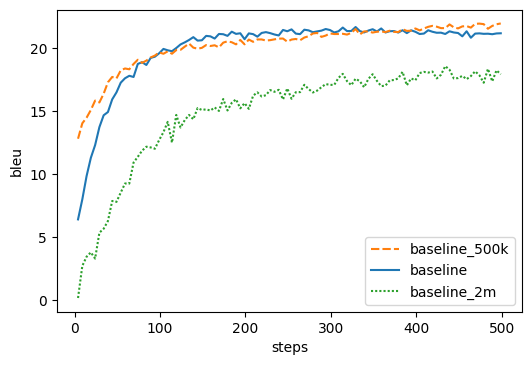
\includegraphics[width=0.95\textwidth]{img/baseline.png}}
    \centering
    \caption{
        Comparison between baseline models trained with different size of datasets. \texttt{baseline} represents the model trained only using IWSLT; \texttt{baseline\_500k} represents the model trained using IWSLT and WMT with total of 500k sentence pairs; \texttt{baseline\_2m} represents the model trained using IWSLT and WMT with total of 2 million sentence pairs.}
    \label{img:basecomp}
\end{figure}

In this section, we compare the result of the baseline models with the models that are fine-tuned with adapters. From Figure \ref{img:basecomp}, adding more data to the baseline models does not necessarily improve the performance. We suspect the models require more time to train to get better performance. There is a clear gap between \texttt{baseline\_2m} and the rest of the baseline models. \texttt{baseline} and \texttt{baseline\_500k} performs really well from the start while \texttt{baseline\_2m} lag behind. We suspect this is the effect of including more sentences from different domains. \texttt{baseline\_500k} is the best mix given the training time constraint. It provides a balance in between not overfitting in the correct domain and not too much data out of the domain. \texttt{baseline\_2m} shows the impact on domain difference. It does not perform well on IWSLT but it is growing and has a chance to improve the performance further. At a later stage, the \texttt{baseline\_2m} output would deserve manual evaluation, because the lower bleu may not necessarily reflect a lower quality, we can see some of the result in Table \ref{tab:qtvout}.

To see the impact of including adapters, we compare the result on different sizes of pre-training used for the base model. The base models are then fine-tuned with the adapters module on the IWSLT data. As we can see from Figure \ref{img:adpcomp}, BERT achieves the best performance from the earlier steps compared to the rest of the pre-training size. In contrast to the baseline models, we see the benefit of adding more sentences to the pre-training. We can see the performance progression between the model that was trained using 500k data has lower performance than the one using 2 million data. On the other hand, models that only use IWSLT as the pre-training data suffers from performance degradation in the middle of the fine-tuning. We observed that this is due to the gradient explosion on the cross-attention layer. The IWSLT model eventually managed to achieve a similar performance to the 500k model in the later steps.
\begin{figure}[h]
    {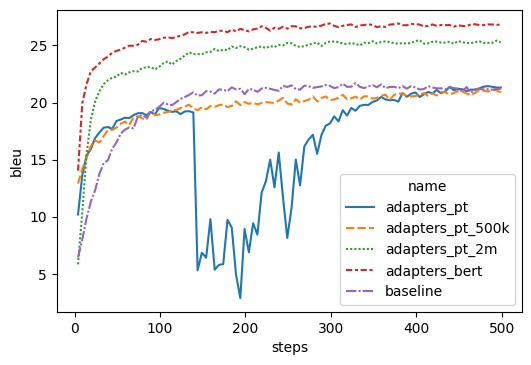
\includegraphics[width=0.95\textwidth]{img/adapterscomparison.png}}
    \centering
    \caption{
        % \XXX{Could you include baseline curve, too? This is rather important for comparison given the lack of the stopping criterion.}
        Comparison between adapters pre-trained with different size of datasets. \texttt{baseline} represents the model trained only using IWSLT; \texttt{adapters\_pt} represents the model pre-trained only using IWSLT; \texttt{adapters\_pt\_500k} represents the model pre-trained using IWSLT and WMT with total of 500k sentence pairs; \texttt{adapters\_pt\_2m} represents the model pre-trained using IWSLT and WMT with total of 2 million sentence pairs; \texttt{adapters\_bert} represents the model that uses BERT weights.}
    \label{img:adpcomp}
\end{figure}

\begin{table*}[]
    \centering
    \begin{tabular}{l}
        \hline
        \multicolumn{1}{c}{\textbf{Random Weights + Adapters}} \\ \hline
        \begin{tabular}[c]{@{}l@{}}\textbf{input}: wir tanzen im tempel und werden zu gott. \& quot ;\\ \textbf{prediction}:we \& apos ; re going to be able to become god. \& quot ;\end{tabular}                              \\ \hline
        \begin{tabular}[c]{@{}l@{}}\textbf{input}: aber gleichzeitig hatten sie eine klare kenntnis des waldes, die erstaunlich war.\\ \textbf{prediction}:but at the same time, they had a clear of the audience who was amazing..\end{tabular}                              \\ \hline
        \begin{tabular}[c]{@{}l@{}}\textbf{input}: es ist so wunderbar. ihr musst es beschutzen. \& quot ;\\ \textbf{prediction}:it \& apos ; s wonderful. you have to protect it. \& quot ;\end{tabular}                              \\ \hline
    \end{tabular}
    \caption{Prediction results from randomly set pre-trained model fine-tuned with adapters}
    \label{tab:qtrand}
\end{table*}

\section{Random and Shuffled Pre-training Weights}
We can see from Figure \ref{img:shfrndcmp} that the performance of the model that uses random weights as the pre-training model is more stable than the one using shuffled BERT weights. Both of the shuffled BERT models suffer from gradient explosion similar to the IWSLT model we show in the previous section. Although the performance of the random model is still below the baseline model, it is interesting to see that only fine-tuning adapters and the cross-attention layer manage to achieve a reasonable BLEU score, considering that the pre-training models do not contain any meaningful information.
\begin{figure}[h]
    {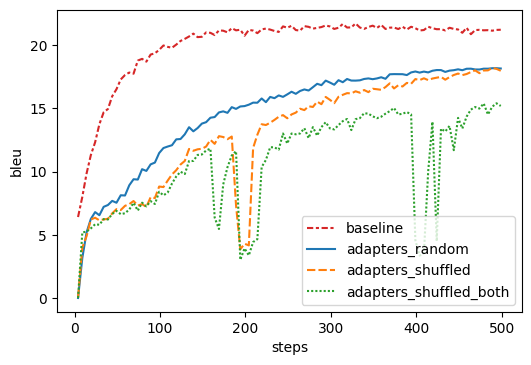
\includegraphics[width=0.95\textwidth]{img/randomshuffled.png}}
    \centering
    \caption{Comparison between adapters using shuffled BERT and random weights as the pre-trained models. \texttt{baseline} represents the model trained only using IWSLT; \texttt{adapters\_random} represents the model pre-trained only using random weights; \texttt{adapters\_shuffled} represents the model pre-trained using column-wise shuffled BERT model; \texttt{adapters\_shuffled\_both} represents the model pre-trained using shuffled BERT model.}
    \label{img:shfrndcmp}
\end{figure}

\section{Random Pretraining vs. Out-of-Domain Data}
We further analyze the random weights by comparing the result with the best performing, baseline, and transformer models we pre-trained ourselves. From Figure \ref{img:rndbslcmp}, we can see that the performance of the random model achieves a similar result to the baseline model that uses 2 million training sentence pairs. While the performance is still far from the baseline that is trained using only IWSLT data, this result shows the base model's structure helps the adapter achieve a meaningful performance with very small weights required for the fine-tuning.

We perform a quick check to the output of the model in Table \ref{tab:qtrand}. We can see from the first two lines that the model hash difficulty to capture complex phrases. On the first row, the model missed \textbf{tanzen im tempel} which means \textbf{dancing in the temple}. For the second row, the model confuses \textbf{knowledge of the forest} and output \textbf{audience instead}. Furthermore, the model also does not translate the word \textbf{kenntnis} and makes the translation unclear since the object of the sentence is missing. Despite those mistakes, the model still can capture simple sentences as shown on the third row. Another observation that we noticed in the generated output is the tokenization of \texttt{\&quot\;} and \texttt{\&amp\;}. Instead of being treated as a single token, the tokenizer treats the token as three different subword token. We notice that this is due to the inavailability of the aforementioned token in the pre-trained BERT vocabulary.


\begin{figure}[h]
    {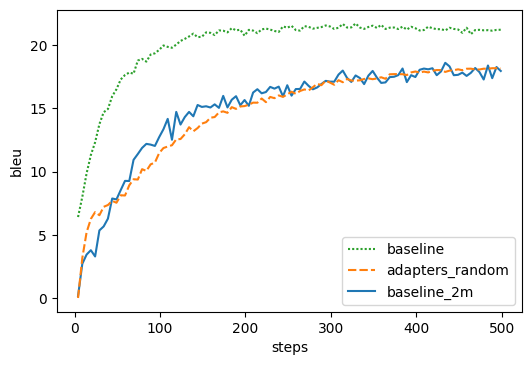
\includegraphics[width=0.95\textwidth]{img/random.png}}
    \centering
    \caption{Comparison between pre-trained random weights and baseline model. \texttt{baseline} represents the model trained only using IWSLT; \texttt{baseline\_2m} represents the baseline model trained with a combination of IWSLT and WMT sentence pairs; \texttt{adapters\_random} represents the model pre-trained only using random weights; \texttt{adapters\_pt\_2m} represents the model pre-trained using IWSLT and WMT with total of 2 million sentence pairs; \texttt{adapters\_bert} represents the model that uses BERT weights}
    \label{img:rndbslcmp}
\end{figure}

\section{Qualitative Comparison}
\begin{table*}[]
    \begin{tabular}{|l|l|l|}
        \hline
        \multicolumn{1}{|c|}{\textbf{Baseline IWSLT}}        &
        \multicolumn{1}{c|}{\textbf{IWSLT + WMT (total 2m)}} &
        \multicolumn{1}{c|}{\textbf{BERT + Adapters}}          \\ \hline
        \begin{tabular}[c]{@{}l@{}}\textbf{input}: erinnerst du dich an\\ den patienten\\ mit dem gereizten rachen? \\ \textbf{prediction}: do you remember\\ reading to the patients? on the\end{tabular}                            &
        \begin{tabular}[c]{@{}l@{}}\textbf{input}: erinnerst du dich an\\ den patienten\\ mit dem gereizten rachen? \\ \textbf{prediction}: do you remember\\ the patient with the tingling\\ revenge?\end{tabular}                           &
        \begin{tabular}[c]{@{}l@{}}\textbf{input}: erinnerst du dich an\\ den patienten\\ mit dem gereizten rachen? \\ \textbf{prediction}: remember the\\ patient with\\ the bruised remorse?\end{tabular}                             \\ \hline
        \begin{tabular}[c]{@{}l@{}}\textbf{input}: großartig, sagte ich.\\ legte auf.\\ \textbf{prediction}: great, i said.\\ got up..\end{tabular}                           &
        \begin{tabular}[c]{@{}l@{}}\textbf{input}: großartig, sagte ich.\\ legte auf.\\ \textbf{prediction}: great, i said.\\ put on..\end{tabular}                           &
        \begin{tabular}[c]{@{}l@{}}\textbf{input}: großartig, sagte ich.\\ legte auf.\\ \textbf{prediction}: great, i said.\\ put it down.\end{tabular}                             \\ \hline
        \begin{tabular}[c]{@{}l@{}}\textbf{input}: - - aber in unserer\\ entdeckung der welt, haben\\ wir alle arten unterschiedlicher\\ methoden.\\ \textbf{prediction}: but in our discovery\\ of the world, we \& apos ;\\ ve got all sorts of different\end{tabular}                           &
        \begin{tabular}[c]{@{}l@{}}\textbf{input}: - - aber in unserer\\ entdeckung der welt, haben\\ wir alle arten unterschiedlicher\\ methoden.\\ \textbf{prediction}: - - but in our discovery\\ of the world, we have\\ all kinds of different methods.\end{tabular}                           &
        \begin{tabular}[c]{@{}l@{}}\textbf{input}: - - aber in unserer\\ entdeckung der welt, haben\\ wir alle arten unterschiedlicher\\ methoden.\\ \textbf{prediction}: but in our discovery\\ of the world, we have\\ all sorts of different ways of doing\\ things.\end{tabular}                             \\ \hline
    \end{tabular}
    \caption{Prediction results from 1) Baseline model trained with only IWSLT data; 2) Pre-trained model with adapters where we pre-train the model with IWSLT and WMT with a total of 2 million pre-training data; 3) BERT with adapters.}
    \label{tab:qtvout}
\end{table*}
We perform a sanity check to compare the generated results on some of our models. This sanity check is to check the errors produced by the models on different techniques.
From Table \ref{tab:qtvout}, we can see for the first example none of the models managed to generate the correct result. However, BERT + adapters and 2 million pre-trained base models manage to generate the proper context where the result is still discussing \textbf{the patient}. The wrong part is when the model generates an incorrect translation regarding the patient's disease. The second example shows that the BERT + adapters create the correct and better output than the other models. The final example shows that BERT + adapters generate an interesting output where it manages to remove unimportant characters such as \texttt{--} and produce readable output. There may be a slightly different opinion on this example as the 2 million pre-trained base model generate a more concise output.
